\section[Lagrange Multipliers]{Lagrange Multipliers}

\begin{frame}{Formulation of an Optimization Problem}
	An \textbf{optimization} problem consists of finding the maximum or minimum value of a function $f(x)$, or alternatively, finding the value of the \textbf{argument} $x$ that maximizes or minimizes this same function. Suppose we are looking for the argument $x$ of a function $f$ that we wish to maximize; the problem is written as follows: \\
	\begin{equation}
		\begin{cases}
			f: \R^p \to \R \\
			\argmax{x \in \R^p} f(x)
		\end{cases}
		\nonumber
	\end{equation}
\end{frame}

\begin{frame}{Formulation of a Constrained Optimization Problem}
	A constrained optimization problem forces the argument $x$ to satisfy certain conditions in order to be a \textbf{feasible} solution to the problem. Such a condition is, for example, an \textbf{equality constraint} like $g(x) = 0$. If we add this type of constraint to our previous problem, the formalization becomes:
	\begin{equation}
		\begin{cases}
			f: \R^p \to \R \\
			g: \R^p \to \R \\
			\argmax{x \in \R^p} f(x) \quad \text{subject to} \quad g(x) = 0
		\end{cases}
		\nonumber
	\end{equation}
	\pause
	Note: In the following formulations, the phrase \textit{subject to} will simply be abbreviated as \textit{s.t.}
\end{frame}

\begin{frame}{Statement of Lagrange Multipliers}
	\begin{block}{Theorem: Lagrange Multipliers}
		Let there be a problem of finding the argument $x \in \R^p$ that maximizes a function $f: \R^p \to \R$ subject to an equality constraint $g(x) = 0$ where $g: \R^p \to \R$:
		\begin{equation}
			\argmax{x} f(x) \quad \text{s.t.} \quad g(x) = 0
			\nonumber
		\end{equation}
		We introduce a function called the \textbf{Lagrangian}, denoted by $\mathcal{L}: \R^p \times \R \to \R$, and a \textbf{multiplier}, denoted by $\lambda \in \R$, such that:
		\begin{equation}
			\mathcal{L}(x, \lambda) = f(x) - \lambda g(x)
			\nonumber
		\end{equation}
		A solution to this constrained optimization problem $(x^*, \lambda^*)$ is obtained when the derivatives of the Lagrangian vanish:
		\begin{equation}
			\begin{cases}
				\nabla_x \mathcal{L}(x^*, \lambda^*) = 0          & \text{stationarity condition} \\
				\nabla_{\lambda} \mathcal{L}(x^*, \lambda^*) = 0  & \text{feasibility condition}
				\nonumber
			\end{cases}
		\end{equation}
	\end{block}
\end{frame}

\begin{frame}{Interpretation of Lagrange Multipliers}
	In the previous theorem:
	\begin{itemize}
		\item $\nabla$ represents the \textbf{gradient} operator:
		\begin{equation}
			\nabla_x = \begin{pmatrix}
				\frac{\partial}{\partial{x_1}} \\
				\frac{\partial}{\partial{x_2}} \\
				\vdots \\
				\frac{\partial}{\partial{x_p}} \\
			\end{pmatrix}; \quad \nabla_{\lambda} = \frac{\partial}{\partial{\lambda}}
			\nonumber
		\end{equation}
		\pause
		\item The first condition (stationarity) ensures that we are looking for a local extremum for $f$. It also guarantees the collinearity of the gradients $\nabla_x$ of $f(x)$ and $g(x)$, and therefore the tangency of the level curves (or surfaces) of functions $f$ and $g$ at the optimal point $(x^*, \lambda^*)$.
	\end{itemize}
\end{frame}

\begin{frame}{Interpretation of Lagrange Multipliers}
	In the previous theorem:
	\begin{itemize}
		\item The second condition (feasibility) guarantees that the constraint $g(x) = 0$ is satisfied; indeed: $\nabla_{\lambda}\mathcal{L}(x, \lambda) = 0 \iff g(x) = 0$
		\pause
		\item The method of Lagrange multipliers generally requires solving a nonlinear system of equations.
		\pause
		\item Since the method of Lagrange multipliers provides access to the feasible extrema of $f$, it is necessary to verify which values of $(x, \lambda)$ actually maximize $f(x)$, given that we seek, in our example, to maximize $f(x)$ under constraint.
	\end{itemize}
\end{frame}

\begin{frame}{Geometric Interpretation of Lagrange Multipliers}
	\begin{figure}
		\centering
		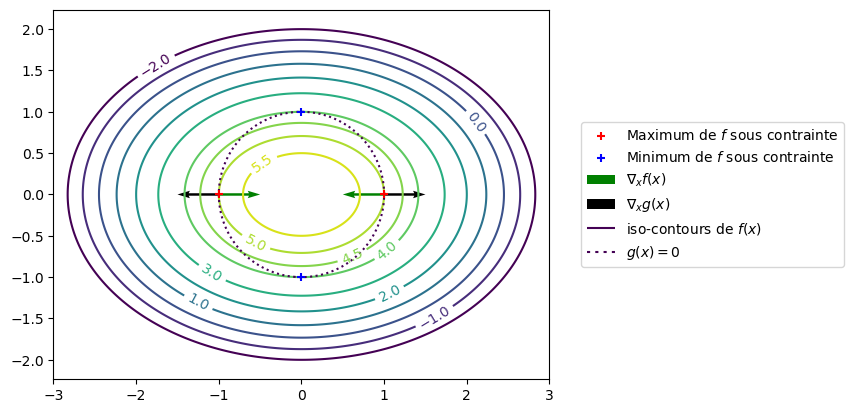
\includegraphics[width=0.95\linewidth]{Images/multiplicateurs_lagrange}
		\label{fig:multiplicateurs_lagrange}
	\end{figure}
\end{frame}